%%%%%%%%%%%%%%%%%%%%%%%%%%%%%%%%%%%%%%%%%%%%%%%%%%%%%%%%%%%%%%%%%%%%%%%%%%%%%%%%%%%%%%%%
\chapter{Three-Dimensional Kitaev Models}
\label{appendix:ThreeDimensionalKitaevModels}
%%%%%%%%%%%%%%%%%%%%%%%%%%%%%%%%%%%%%%%%%%%%%%%%%%%%%%%%%%%%%%%%%%%%%%%%%%%%%%%%%%%%%%%%
%
%
%%%%%%%%%%%%%%%%%%%%%%%%%%%%%%%%%%%%%%%%%%%%%%%%%%%%%%%%%%%%%%%%%%%%%%%%%%%%%%%%%%%%%%%%
\section{Lattice (8,3)a}
\label{appendix:ThreeDimensionalKitaevModels_8_3a}
%%%%%%%%%%%%%%%%%%%%%%%%%%%%%%%%%%%%%%%%%%%%%%%%%%%%%%%%%%%%%%%%%%%%%%%%%%%%%%%%%%%%%%%%
%
%
Lattice (8,3)a possesses three loop operators of length 8 and three of length 14 per unit cell.
These six loop operators may be combined to form three closed volumes leading to only \textit{three} independent loop operators per unit cell.
One of these closed volumes is illustrated in Figure~\ref{fig:appendix_8_3aVolume}.
The remaining two volumes are related by a threefold screw rotation.
The smallest vison loop in this lattice threads two plaquettes of length 8 as well as several plaquettes of length 14, as visualized in Figure~\ref{fig:appendix_8_3aVison}.
%
\begin{figure}[ht!]
	\centering
	\includegraphics[width=0.8\linewidth]{./appendixThreeDimensionalKitaevModels/8_3aVolume.png}
	\caption{
		Loop operators of lattice (8,3)a forming a volume constraint.
	}
	\label{fig:appendix_8_3aVolume}
\end{figure}
%
%
\begin{figure}[ht!]
	\centering
	\includegraphics[width=0.8\linewidth]{./appendixThreeDimensionalKitaevModels/8_3aVison.png}
	\caption{
		Vison excitation of lattice (8,3)a threading two plaquettes of length 8.
		In addition, it threads several plaquettes of length 14, two examples of which are depicted on the right, shaded in magenta.
		The flipped bond operator is pictured in red.
	}
	\label{fig:appendix_8_3aVison}
\end{figure}
%


%
%
%%%%%%%%%%%%%%%%%%%%%%%%%%%%%%%%%%%%%%%%%%%%%%%%%%%%%%%%%%%%%%%%%%%%%%%%%%%%%%%%%%%%%%%%
\section{Lattice (8,3)b}
\label{appendix:ThreeDimensionalKitaevModels_8_3b}
%%%%%%%%%%%%%%%%%%%%%%%%%%%%%%%%%%%%%%%%%%%%%%%%%%%%%%%%%%%%%%%%%%%%%%%%%%%%%%%%%%%%%%%%
%
%
Lattice (8,3)b possesses three loop operators of length 8 and one of length 12 per unit cell.
These four loop operators may be combined to form a closed volume leading to only \textit{three} independent loop operators per unit cell.
This closed volume is illustrated in Figure~\ref{fig:appendix_8_3bVolume}.
The smallest vison loop in this lattice threads two plaquettes of length 8 and two of length 12 and is visualized in Figure~\ref{fig:appendix_8_3bVison}.
%
\begin{figure}[ht!]
	\centering
	\includegraphics[width=0.8\linewidth]{./appendixThreeDimensionalKitaevModels/8_3bVolume.png}
	\caption{
		Loop operators of lattice (8,3)b forming a volume constraint.
		The loop operators in the bottom row are related to those in the top row by lattice translation vectors.
	}
	\label{fig:appendix_8_3bVolume}
\end{figure}
%
%
\begin{figure}[ht!]
	\centering
	\includegraphics[width=0.8\linewidth]{./appendixThreeDimensionalKitaevModels/8_3bVison.png}
	\caption{
		Vison excitation of lattice (8,3)b threading four plaquettes -- two of length 8 and two of length 12, shaded in yellow and magenta, respectively.
		The flipped bond operator is pictured in red.
	}
	\label{fig:appendix_8_3bVison}
\end{figure}
%


%
%
%%%%%%%%%%%%%%%%%%%%%%%%%%%%%%%%%%%%%%%%%%%%%%%%%%%%%%%%%%%%%%%%%%%%%%%%%%%%%%%%%%%%%%%%
\section{Lattice (8,3)c}
\label{appendix:ThreeDimensionalKitaevModels_8_3c}
%%%%%%%%%%%%%%%%%%%%%%%%%%%%%%%%%%%%%%%%%%%%%%%%%%%%%%%%%%%%%%%%%%%%%%%%%%%%%%%%%%%%%%%%
%
%
Lattice (8,3)c possesses six loop operators of length 8 and one of length 18 per unit cell.
These seven loop operators may be combined to form three closed volumes leading to only \textit{four} independent loop operators per unit cell.
Two of these closed volumes are constructed only from loops of length 8 and are related to each other by a sixfold screw rotation.
The remaining volume is constructed from six loops of length 8 and two of length 18.
This larger closed volume and one of the smaller closed volumes are illustrated in Figure~\ref{fig:appendix_8_3cVolume}.
The smallest vison loop in this lattice threads four plaquettes of length 8 and several plaquettes of length 18 as visualized in Figure~\ref{fig:appendix_8_3cVison}.
%
\begin{figure}[ht!]
	\centering
	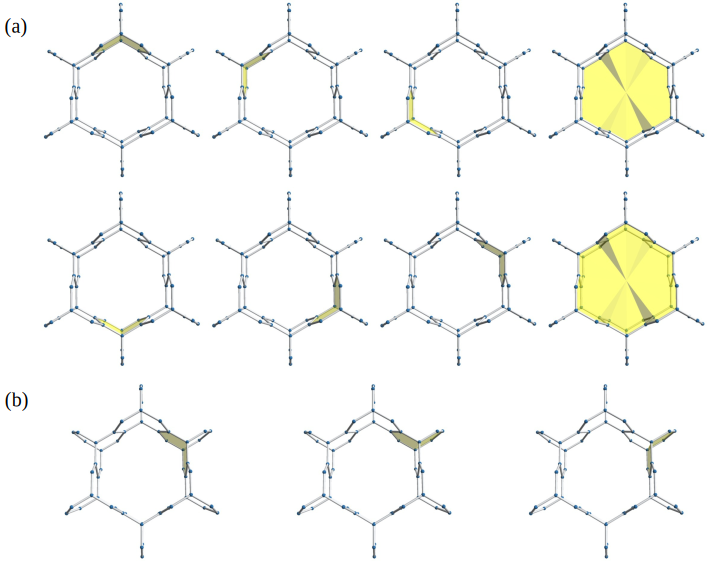
\includegraphics[width=0.8\linewidth]{./appendixThreeDimensionalKitaevModels/8_3cVolume.pdf}
	\caption{
		Loop operators of lattice (8,3)c forming two unique volume constraints in (a) and (b).
	}
	\label{fig:appendix_8_3cVolume}
\end{figure}
%
%
\begin{figure}[ht!]
	\centering
	\includegraphics[width=0.8\linewidth]{./appendixThreeDimensionalKitaevModels/8_3cVison.png}
	\caption{
		Vison excitation of lattice (8,3)c threading four plaquettes of length 8, shaded in magenta.
		In addition, it threads several plaquettes of length 18, two examples of which are depicted here, shaded in magenta.
		The flipped bond operator is pictured in red.
	}
	\label{fig:appendix_8_3cVison}
\end{figure}
%


%
%
%%%%%%%%%%%%%%%%%%%%%%%%%%%%%%%%%%%%%%%%%%%%%%%%%%%%%%%%%%%%%%%%%%%%%%%%%%%%%%%%%%%%%%%%
\section{Lattice (8,3)n}
\label{appendix:ThreeDimensionalKitaevModels_8_3n}
%%%%%%%%%%%%%%%%%%%%%%%%%%%%%%%%%%%%%%%%%%%%%%%%%%%%%%%%%%%%%%%%%%%%%%%%%%%%%%%%%%%%%%%%
%
%
Lattice (8,3)n possesses six loop operators of length 8, four of length 10, and two of length 12 per unit cell.
These twelve loop operators may be combined to form four closed volumes leading to only \textit{eight} independent loop operators per unit cell.
These closed volumes are illustrated in Figure~\ref{fig:appendix_8_3nVolume}.
The smallest vison loop in this lattice threads two plaquettes of length 8 and two of length 10 and is visualized in Figure~\ref{fig:appendix_8_3nVison}.
%
\begin{figure}[ht!]
	\centering
	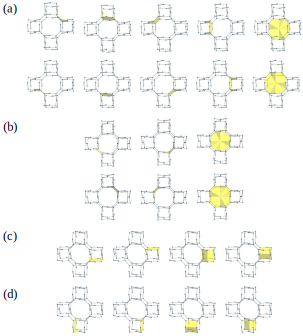
\includegraphics[width=0.8\linewidth]{./appendixThreeDimensionalKitaevModels/8_3nVolume.pdf}
	\caption{
		Loop operators of lattice (8,3)n forming four unique volume constraints in (a), (b), (c) and (d).
	}
	\label{fig:appendix_8_3nVolume}
\end{figure}
%
%
\begin{figure}[ht!]
	\centering
	\includegraphics[width=0.8\linewidth]{./appendixThreeDimensionalKitaevModels/8_3nVison.png}
	\caption{
		Vison excitation of lattice (8,3)n threading two plaquettes of length 8 and two plaquettes of length 10, shaded in yellow and magenta, respectively.
		The flipped bond operator is pictured in red.
	}
	\label{fig:appendix_8_3nVison}
\end{figure}
%


%
%
%%%%%%%%%%%%%%%%%%%%%%%%%%%%%%%%%%%%%%%%%%%%%%%%%%%%%%%%%%%%%%%%%%%%%%%%%%%%%%%%%%%%%%%%
\section{Lattice (9,3)a}
\label{appendix:ThreeDimensionalKitaevModels_9_3a}
%%%%%%%%%%%%%%%%%%%%%%%%%%%%%%%%%%%%%%%%%%%%%%%%%%%%%%%%%%%%%%%%%%%%%%%%%%%%%%%%%%%%%%%%
%
%
Lattice (9,3)a has eight loops of length 9 and one loop of length 12 per unit cell.
These nine loop operators may be combined to form two closed volumes, each of which shares a loop of length 12, leading to only \textit{six} independent loop operators of length 9 per unit cell.
These closed volumes are illustrated in Figure~\ref{fig:appendix_9_3aVolume}.
The smallest vison loop in this lattice threads four plaquettes of length 9 and is visualized in Figure~\ref{fig:appendix_9_3aVison}.
%
\begin{figure}[ht!]
	\centering
	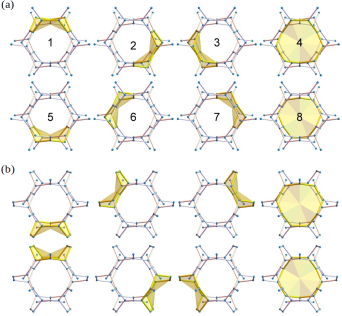
\includegraphics[width=0.8\linewidth]{./appendixThreeDimensionalKitaevModels/9_3aVolume.pdf}
	\caption{
		Loop operators of lattice (9,3)a forming two unique volume constraints in (a) and (b).
	}
	\label{fig:appendix_9_3aVolume}
\end{figure}
%
%
\begin{figure}[ht!]
	\centering
	\includegraphics[width=0.8\linewidth]{./appendixThreeDimensionalKitaevModels/9_3aVison.png}
	\caption{
		Vison excitation of lattice (9,3)a threading four plaquettes of length 9.
		The flipped bond operator is pictured in red.
	}
	\label{fig:appendix_9_3aVison}
\end{figure}
%


%
%
%%%%%%%%%%%%%%%%%%%%%%%%%%%%%%%%%%%%%%%%%%%%%%%%%%%%%%%%%%%%%%%%%%%%%%%%%%%%%%%%%%%%%%%%
\section{Lattice (10,3)a}
\label{appendix:ThreeDimensionalKitaevModels_10_3a}
%%%%%%%%%%%%%%%%%%%%%%%%%%%%%%%%%%%%%%%%%%%%%%%%%%%%%%%%%%%%%%%%%%%%%%%%%%%%%%%%%%%%%%%%
%
%
Lattice (10,3)a possesses six loop operators of length 10 per unit cell.
These six loop operators may be combined to form four closed volumes leading to only \textit{two} independent loop operators per unit cell.
One of these closed volumes is illustrated in Figure~\ref{fig:appendix_10_3aVolume}.
The smallest vison loop in this lattice threads ten plaquettes of length 10 and is visualized in Figure~\ref{fig:appendix_10_3aVison}.
%
\begin{figure}[ht!]
	\centering
	\includegraphics[width=0.8\linewidth]{./appendixThreeDimensionalKitaevModels/10_3aVolume.png}
	\caption{
		Loop operators of lattice (10,3)a forming a volume constraint.
	}
	\label{fig:appendix_10_3aVolume}
\end{figure}
%
%
\begin{figure}[ht!]
	\centering
	\includegraphics[width=0.8\linewidth]{./appendixThreeDimensionalKitaevModels/10_3aVison.png}
	\caption{
		Vison excitation of lattice (10,3)a threading ten plaquettes of length 10.
		The flipped bond operator is pictured in red.
	}
	\label{fig:appendix_10_3aVison}
\end{figure}
%


\pagebreak
%
%
%%%%%%%%%%%%%%%%%%%%%%%%%%%%%%%%%%%%%%%%%%%%%%%%%%%%%%%%%%%%%%%%%%%%%%%%%%%%%%%%%%%%%%%%
\section{Lattice (10,3)b}
\label{appendix:ThreeDimensionalKitaevModels_10_3b}
%%%%%%%%%%%%%%%%%%%%%%%%%%%%%%%%%%%%%%%%%%%%%%%%%%%%%%%%%%%%%%%%%%%%%%%%%%%%%%%%%%%%%%%%
%
%
Lattice (10,3)b possesses four loop operators of length 10 per unit cell.
These four loop operators can be combined to form two closed volumes, leading to only \textit{two} independent loop operators per unit cell.
One of these closed volumes is illustrated in Figure~\ref{fig:appendix_10_3bVolume}.
The remaining volume is related by a twofold screw rotation.
The smallest vison loop in this lattice threads six plaquettes of length 10 and is visualized in Figure~\ref{fig:appendix_10_3bVison}.
%
\begin{figure}[ht!]
	\centering
	\includegraphics[width=0.8\linewidth]{./appendixThreeDimensionalKitaevModels/10_3bVolume.png}
	\caption{
		Loop operators of lattice (10,3)b forming a volume constraint.
	}
	\label{fig:appendix_10_3bVolume}
\end{figure}
%
%
\begin{figure}[ht!]
	\centering
	\includegraphics[width=0.8\linewidth]{./appendixThreeDimensionalKitaevModels/10_3bVison.png}
	\caption{
		Vison excitation of lattice (10,3)b threading six plaquettes of length 10.
		The flipped bond operator is pictured in red.
	}
	\label{fig:appendix_10_3bVison}
\end{figure}
%


\pagebreak
%
%
%%%%%%%%%%%%%%%%%%%%%%%%%%%%%%%%%%%%%%%%%%%%%%%%%%%%%%%%%%%%%%%%%%%%%%%%%%%%%%%%%%%%%%%%
\section{Lattice (10,3)c}
\label{appendix:ThreeDimensionalKitaevModels_10_3c}
%%%%%%%%%%%%%%%%%%%%%%%%%%%%%%%%%%%%%%%%%%%%%%%%%%%%%%%%%%%%%%%%%%%%%%%%%%%%%%%%%%%%%%%%
%
%
Lattice (10,3)c possesses three loop operators of length 10 and three of length 12 per unit cell.
These six loop operators can be combined to form three closed volumes, leading to only \textit{three} independent loop operators per unit cell.
One of these closed volumes is illustrated in Figure~\ref{fig:appendix_10_3cVolume}.
Note that this particular visualization obscures the fact that different loop operators of length 12 are symmetry related.
The remaining two volumes are related by a threefold screw rotation.
The smallest vison loop in this lattice threads three plaquettes of length 10 and eleven of length 12 and is visualized in Figure~\ref{fig:appendix_10_3cVison}.
%
\begin{figure}[ht!]
	\centering
	\includegraphics[width=0.8\linewidth]{./appendixThreeDimensionalKitaevModels/10_3cVolume.png}
	\caption{
		Loop operators of lattice (10,3)c forming a volume constraint.
	}
	\label{fig:appendix_10_3cVolume}
\end{figure}
%
%
\begin{figure}[ht!]
	\centering
	\includegraphics[width=0.8\linewidth]{./appendixThreeDimensionalKitaevModels/10_3cVison.png}
	\caption{
		Vison excitation of lattice (10,3)c threading three plaquettes of length 10, shaded in yellow.
		In addition, eleven plaquettes of length 12 are excited -- four examples of such plaquettes are shown in the bottom row, shaded in magenta.
		The flipped bond operator is pictured in red.
	}
	\label{fig:appendix_10_3cVison}
\end{figure}
%

As mentioned in Section~\ref{section:chapter05_10_3c}, in order to accommodate a gauge \textit{Ansatz} compatible with the ground state flux sector, the unit cell must be enlarged in the 010-direction to a 12 site unit cell.
The sites have been relabeled for the enlarged unit cell, which is depicted in Figure~\ref{fig:appendix_10_3cEnlargedUnitCell}.
%
\begin{figure}[tb]
	\centering
	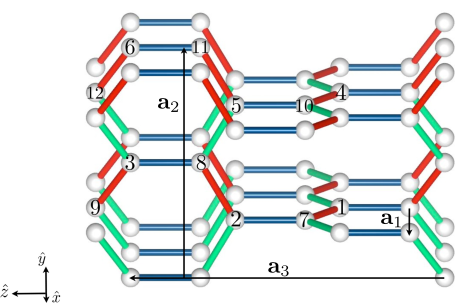
\includegraphics[width=0.6\linewidth]{./appendixThreeDimensionalKitaevModels/10_3cEnlargedUnitCell.pdf}
	\caption{
		Visualization of the Kitaev couplings, unit cell and translation vectors for the enlarged unit cell of lattice (10,3)c.
	}
	\label{fig:appendix_10_3cEnlargedUnitCell}
\end{figure}
%
